% !TEX program = xelatex
\documentclass[10pt,letterpaper,twocolumn]{article}

% === PAGE ===
\usepackage[top=0.75in,bottom=0.75in,left=0.75in,right=0.75in,footskip=12pt]{geometry}

% === FONTS ===
\usepackage{fontspec}
\usepackage{unicode-math}
\setmainfont{Latin Modern Roman}[
  Extension=.otf,
  UprightFont=lmroman10-regular,
  BoldFont=lmroman10-bold,
  ItalicFont=lmroman10-italic,
  BoldItalicFont=lmroman10-bolditalic,
]
\setsansfont{Latin Modern Sans}[
  Extension=.otf,
  UprightFont=lmsans10-regular,
  BoldFont=lmsans10-bold,
  ItalicFont=lmsans10-oblique,
  BoldItalicFont=lmsans10-boldoblique,
]
\setmonofont{Latin Modern Mono}[
  Extension=.otf,
  UprightFont=lmmono10-regular,
  BoldFont=lmmonolt10-bold,
  ItalicFont=lmmono10-italic,
  Scale=0.85,
]
\newfontfamily\acbold{ywft-processing-bold}[
  Path=../../system/public/type/webfonts/,
  Extension=.ttf
]

% === PACKAGES ===
\usepackage{xcolor}
\usepackage{titlesec}
\usepackage{enumitem}
\usepackage{booktabs}
\usepackage{tabularx}
\newcolumntype{Y}{>{\RaggedRight\arraybackslash}X}
\usepackage{fancyhdr}
\usepackage{hyperref}
\usepackage{xurl}
\usepackage{graphicx}
\graphicspath{{./}{figures/}}
\usepackage{ragged2e}
\usepackage{microtype}
\usepackage[font=footnotesize]{caption}
\usepackage{subcaption}
\usepackage{natbib}
\usepackage{tikz}
\usetikzlibrary{arrows.meta,calc,positioning}
\usepackage{../ac-source-bundle}

% === COLORS ===
\definecolor{acpink}{RGB}{180,72,135}
\definecolor{acpurple}{RGB}{120,80,180}
\definecolor{acdark}{RGB}{64,56,74}
\definecolor{acgray}{RGB}{119,119,119}
\definecolor{acblue}{RGB}{42,100,212}
\definecolor{acgreen}{RGB}{52,140,84}

\hypersetup{
  colorlinks=true,
  linkcolor=acpurple,
  urlcolor=acpurple,
  citecolor=acpurple,
  pdfauthor={@jeffrey},
  pdftitle={Eat the Right Answer: Gaming and Education, Tested Against What Aesthetic.Computer Built},
}

% === SECTIONS ===
\titleformat{\section}{\normalfont\bfseries\normalsize\uppercase}{\thesection.}{0.5em}{}
\titlespacing{\section}{0pt}{1.2em}{0.3em}
\titleformat{\subsection}{\normalfont\bfseries\small}{\thesubsection}{0.5em}{}
\titlespacing{\subsection}{0pt}{0.8em}{0.2em}

% === RUNNING MATTER ===
\pagestyle{fancy}
\fancyhf{}
\renewcommand{\headrulewidth}{0pt}
\fancyfoot[C]{\footnotesize\thepage}
\setlist[itemize]{nosep,leftmargin=1.2em,itemsep=0.1em}
\setlist[enumerate]{nosep,leftmargin=1.2em}
\setlength{\columnsep}{1.8em}
\setlength{\parindent}{1em}
\setlength{\parskip}{0.3em}
\tolerance=800
\emergencystretch=1em
\hyphenpenalty=50
\raggedbottom

\newcommand{\acdot}{{\color{acpink}.}}
\newcommand{\ac}{Aesthetic{\acdot}Computer}
\newcommand{\code}[1]{\texttt{#1}}
\newcommand{\term}[1]{``#1''}
\newcommand{\coverplate}{%
  \begin{tikzpicture}
    \node[inner sep=0pt,outer sep=0pt,rounded corners=14pt,fill=acpink!6]
      {
\includegraphics[width=0.40\textwidth]{figures/cover}};
  \end{tikzpicture}%
}

\InputIfFileExists{version}{}{%
  \providecommand{\paperhash}{dev}\providecommand{\paperrev}{?}}

\newcommand{\plang}[2]{\href{https://papers.aesthetic.computer/gaming-education-26-arxiv#2.pdf}{\color{acgray}#1}}
\newcommand{\planghere}[1]{{\bfseries\color{acpink}#1}}
\newcommand{\plangsep}{{\color{acgray!60}\,\textperiodcentered\,}}

\begin{document}

\twocolumn[{%
\begin{center}
{\acbold\fontsize{26pt}{30pt}\selectfont\color{acdark} Eat the Right Answer}\par
\vspace{0.45em}
{\itshape\fontsize{14pt}{17pt}\selectfont\color{acpink} Gaming and Education, Tested Against What \ac{} Built}\par
\vspace{0.5em}
\coverplate\par
\vspace{0.5em}
{\small\color{acgray} \href{https://prompt.ac/@jeffrey}{@jeffrey} \,\textperiodcentered\, \ac{} \,\textperiodcentered\, ORCID \href{https://orcid.org/0009-0007-4460-4913}{0009-0007-4460-4913} \,\textperiodcentered\, September 2026}\par
\vspace{0.45em}
{\footnotesize\sffamily\planghere{EN}\plangsep\plang{DA}{-da}\plangsep\plang{ES}{-es}\plangsep\plang{ZH}{-zh}\plangsep\plang{JA}{-ja}}\par
\vspace{0.55em}
{\color{acpink}\rule{\textwidth}{1.2pt}}
\vspace{0.5em}
\end{center}

\begin{quote}
\small\noindent\textbf{Abstract.}
The claim that games teach is forty years old and usually argued from one of two ends: from the game, by people who love games, or from the classroom, by people who need something to show for the period. This paper argues from the middle, using three objects built inside \ac{} in 2026. The first is the \code{nom} family, eight muncher drills on one 3,182-line engine, whose June paper predicted that the next subject would cost a content table and whose repository history since then is the test of that prediction. The second is the KidLisp card, a two-to-four-line program printed with its output, handed to a UCLA cohort as a score. The third is the oskiewar coach, a spectator process that takes the agent seat on a fighting-game match, never presses a button, and keeps a ledger a model can teach from. I read the three against the literature they descend from, Malone and Habgood on intrinsic integration, Papert and Resnick on construction, Gee and Ito on what games already do, and Vygotsky on the person who watches. The finding is a seam, the same one in all three: a fixed engine, a swappable table of content, and a watcher on the outside. The drill has the first two and no watcher. The card has a human one. The coach is a machine one, four days old. Games teach when the answer is the thing you do, and someone is keeping score of more than the score.
\end{quote}
\vspace{0.5em}
}]

\section{The Question Is Old}
\label{sec:intro}

In 1986 a green creature on an Apple~II ate the multiples of three and a generation of American nine-year-olds did arithmetic without noticing~\citep{mecc1986number}. In 1980 Seymour Papert had already argued that the child should be programming the computer and not the other way round~\citep{papert1980mindstorms}. Those two sentences are the whole debate. One side builds the drill and dresses it up. The other side hands over the language and waits. Forty years of gaming-and-education literature is mostly the two sides describing each other's failures.

This paper does not settle that. It looks at three things I actually built and asks which side each one is on, what it borrowed from the other, and what it is missing. The objects are recent and small, which is the point: they are legible all the way down, the repository dates them, and their gaps are on the record.

\begin{itemize}
  \item \textbf{The \code{nom} family} (Section~\ref{sec:nom}), eight muncher drills that share an engine and differ by a table. The June 2026 paper on them made a prediction about how they would grow, and three months of commits either bear it out or do not.
  \item \textbf{KidLisp cards} (Section~\ref{sec:cards}), a program, its source, and its picture on one printed card, taken into a UCLA classroom as a score.
  \item \textbf{The oskiewar coach} (Section~\ref{sec:coach}), a one-file spectator that watches a two-player fighting game and hands a model the ledger.
\end{itemize}

Section~\ref{sec:method} records what was consulted. Section~\ref{sec:traditions} lays out the two traditions and the one thing both of them under-build. Section~\ref{sec:seam} draws the seam the three objects share. Section~\ref{sec:school} asks what a school would need. Section~\ref{sec:limits} says what this paper cannot claim.

\section{Sources and Method}
\label{sec:method}

The Platter consulted for this paper is its own prior work plus the standard literature. On the \ac{} side: \emph{The nom Games}~\citep{scudder2026nom}, \emph{KidLisp Cards}~\citep{scudder2026kidlispcards}, \emph{Get Closed Source Out of Schools}~\citep{scudder2026openschools}, \emph{oskiewar}~\citep{scudder2026oskiewar}, \emph{Pieces Not Programs}~\citep{scudder2026pieces}, \emph{Free Versus Nonfree}~\citep{scudder2026freevsopen}, and the March 2026 proposal to UCLA's \emph{Scores for Social Software} cycle~\citep{sosoft2026proposal}. The repository was inspected on September 19, 2026 at commit \code{37ffe2f962}; every line count, date, and table size below comes from that tree or its \code{git log}~\citep{acrepo2026}. The three screenshots in Figure~\ref{fig:boards} were taken the same day from the live site through headless Chrome at a phone-sized 330$\times$270 CSS pixels; no play was scripted, so each shows the board a player sees a few seconds after arriving, with whichever round the engine dealt. The cover is an edit in the house illustration lineage; its sources are logged beside it.

The literature was read for what it claims, not to prove it was read. Where a claim is contested I say who contests it.

\section{Two Traditions and the Thing Both Skip}
\label{sec:traditions}

Mizuko Ito's cultural history of children's software sorts the field into three genres: \emph{academic} (the drill, sold to anxious parents), \emph{entertainment} (the game, sold to the child), and \emph{construction} (the kit, sold to the idea of the child as maker)~\citep{ito2009engineering}. The sorting is useful because the three genres had different economics, different rhetorics, and mostly different people, and because it names the two poles this paper's objects sit between.

\subsection{The drill, done well}

The academic genre's best defense is not that drilling works but that a particular kind of drill does. Thomas Malone's 1981 theory of intrinsically motivating instruction named the ingredients, challenge, fantasy, and curiosity, and warned that fantasy laid on top of a drill (\emph{extrinsic} fantasy) motivates less than fantasy that is the drill (\emph{intrinsic} fantasy)~\citep{malone1981thinking}. Thirty years later Habgood and Ainsworth tested exactly this, building two versions of the same math game, one where the arithmetic was the core mechanic and one where it interrupted play, and found children chose to play the integrated version longer and learned more from it~\citep{habgood2011motivating}. They called the property \emph{intrinsic integration}. \emph{Number Munchers} had it by accident of design: eating the prime \emph{is} the game~\citep{mecc1986number,mecc1985word}.

That is the drill's whole case, and it is a good one. It is also the whole of what the drill does. Nothing in Malone or Habgood says the child understands why 31 is prime. The integrated drill produces fluency, and fluency is real, and the literature is honest that this is what it produces.

\subsection{The kit, and its promise}

Papert's answer was to remove the drill entirely. In \emph{Mindstorms} the child teaches the turtle, and the powerful idea (recursion, a variable, a procedure) arrives because the child needed it to make the thing~\citep{papert1980mindstorms}. Scratch is that argument shipped at scale, with its design summarized as \term{low floor, high ceiling, wide walls}: easy to start, room to grow, many kinds of project~\citep{resnick2009scratch}. Kafai and Burke's \emph{Connected Code} moves the argument from the individual child to the community, arguing that the point of children programming is participation in a culture of making, not a skill for later~\citep{kafai2014connected}; Peppler and Kafai had already framed creative coding as personal expression rather than preparation~\citep{peppler2009creative}.

The construction genre's honest weakness is the opposite of the drill's. It produces understanding for the children who go through the door and no evidence for the ones who do not, and the door is the hard part. Ito's history records that construction software was the genre parents admired and rarely bought.

\subsection{What games already do}

James Paul Gee's contribution was to stop asking whether games could be made educational and to list the thirty-six things good commercial games already do that schools do not: situate meaning, let the player fail cheaply, hand over identity, and so on~\citep{gee2003video}. Squire took the claim into classrooms with \emph{Civilization} and reported the price: games teach, and they teach slowly, unevenly, and mostly to children who were already inclined~\citep{squire2011video}. Steinkuehler and Duncan found scientific habits of mind in \emph{World of Warcraft} forum posts, which is a finding about the community around a game, not the game~\citep{steinkuehler2008scientific}. Bogost's procedural rhetoric argues that a rule system makes a claim by being played~\citep{bogost2007persuasive}. Huizinga's older point, that play draws a circle inside which ordinary consequences are suspended, is the reason all of this works at all, and Salen and Zimmerman's \emph{Rules of Play} made the circle a design term~\citep{huizinga1938homo,salen2004rules}.

\subsection{The watcher}

Read together, the two traditions and the games literature share an absence. Vygotsky's zone of proximal development is the distance between what a learner can do alone and what they can do with someone more capable beside them~\citep{vygotsky1978mind}. The drill has no one beside the child; it has a score. The kit has, at best, a teacher who happens to be in the room. Gee's games have the guild. Freire's objection to \term{banking} education, the depositing of facts into a passive student, is an objection to a drill with no one watching, and bell hooks's answer is a classroom where the teacher is a person in the room and not a delivery mechanism~\citep{freire1970pedagogy,hooks1994teaching}. Kate Compton and Michael Mateas's \emph{casual creators}, tools whose pleasure is exploration and whose output does not much matter, are the one design category that treats the absence of a judge as a feature~\citep{compton2015casual}.

The three objects below are arranged by how they handle the watcher (Table~\ref{tab:genres}). That turns out to be the axis on which they differ most.

\begin{table}[t]
\small
\centering
\begin{tabularx}{\columnwidth}{@{}>{\RaggedRight\arraybackslash}p{2.05cm} Y Y@{}}
\toprule
\textbf{Ito's genre} & \textbf{Object} & \textbf{Who watches} \\
\midrule
academic & the \code{nom} family: a drill with a table & nobody; a spoken rule and a ranked score \\
\addlinespace
construction & KidLisp cards: a program on a card & a teacher with a deck; the cohort \\
\addlinespace
entertainment & oskiewar with its coach & a process that keeps a ledger for a model \\
\bottomrule
\end{tabularx}
\caption{The three objects sorted by Ito's genres of children's software~\citep{ito2009engineering}, with the column this paper adds: who, if anyone, is watching the learner. The drill is the only one with no watcher at all, which is Freire's complaint about it in one word~\citep{freire1970pedagogy}.}
\label{tab:genres}
\end{table}

\section{The Drill That Admits It}
\label{sec:nom}

\begin{figure*}[t]
\centering
\begin{subfigure}[t]{0.325\textwidth}
  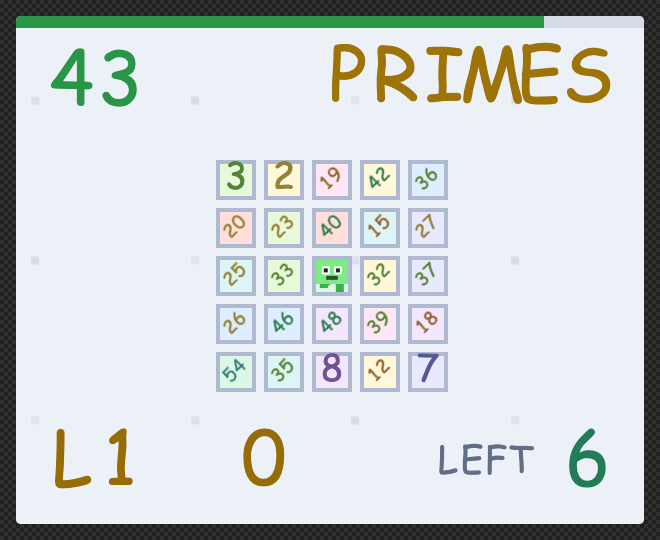
\includegraphics[width=\linewidth]{figures/numbnom}
  \caption{\code{numbnom}: eat the primes; the metronome is a kick.}
  \label{fig:numbnom}
\end{subfigure}\hfill
\begin{subfigure}[t]{0.325\textwidth}
  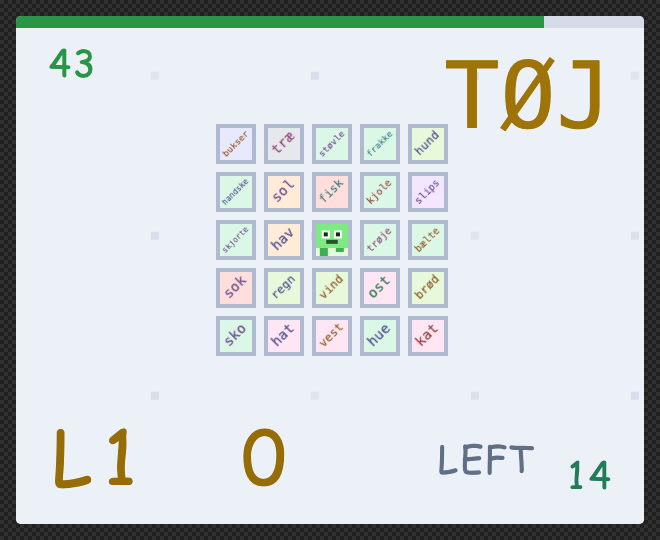
\includegraphics[width=\linewidth]{figures/dannom}
  \caption{\code{dannom}: eat the Danish words for clothes (\emph{t{\o}j}); each munch speaks the English.}
  \label{fig:dannom}
\end{subfigure}\hfill
\begin{subfigure}[t]{0.325\textwidth}
  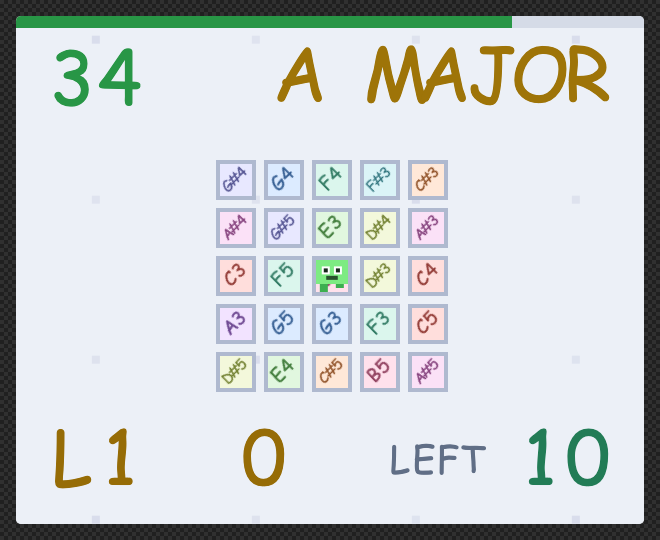
\includegraphics[width=\linewidth]{figures/notenom}
  \caption{\code{notenom}: eat the notes in A major; each munch plays the pitch.}
  \label{fig:notenom}
\end{subfigure}
\caption{Three editions of one engine, captured from the live site on September 19, 2026 a few seconds after load, before any input. The frame is the same in all three: rule at top right, beat-driven timer along the top edge, score at top left, the 5$\times$5 board in the middle, lives and squares remaining at the bottom. Only the cell contents and the munch response differ, which is the paper's claim about the drill made visible: the game is the frame, the subject is the table.}
\label{fig:boards}
\end{figure*}

The \code{nom} games are muncher drills: a 5$\times$5 board, a rule at the top, a green creature you steer onto the squares that satisfy the rule, purple troggles that patrol, and a timer that counts in beats of a metronome you can hear~\citep{scudder2026nom}. Figure~\ref{fig:boards} shows three of them. They are the academic genre without apology. Their paper, written in June 2026 when there were four, claimed that the mechanic was forty years old and good, that the engineering question was where to put the cut between what stays and what varies, and that having put it in the right place, \term{the next subject is already mostly written, it just needs a list.}

That is a testable claim, and the repository has now tested it.

\subsection{What the prediction said}

The June paper's architecture section reported one engine, \code{lib/nom.mjs}, and three thin wrappers, with \code{notenom} as an admitted exception that re-implemented the board and timer on its own. Its limitations section listed four gaps: \code{notenom} was not on the engine, there was no score persistence, the troggles had one personality, and the word lists were short. Its roadmap was a list of tables: more languages, more subjects, procedural rules, multiplayer, and \code{notenom} as an instrument.

\subsection{What happened}

Table~\ref{tab:noms} is the ledger. The engine is 3,182 lines; each of the eight wrappers is between 18 and 21 lines and does nothing but pass a mode name to it. \code{dannom} arrived the same day as the paper. \code{rusnom} and \code{catnom} arrived the next day, and so did the commit that folded \code{notenom} onto the shared engine, closing the paper's first limitation within twenty-four hours of stating it. \code{artnom} arrived six weeks later, and it is the one that stretches the thesis: its content is not a list typed into the engine but a generated catalog, five Getty Art \& Architecture Thesaurus style categories with ten works each, pulled from the Art Institute of Chicago's open API, with rights recorded per object and images left on the museum's IIIF server~\citep{acrepo2026}. A munch reveals the painting. The subject went from \term{a list} to \term{a query,} and the engine did not change shape to receive it.

\begin{table*}[t]
\small
\centering
\begin{tabularx}{\textwidth}{@{}l l Y Y@{}}
\toprule
\textbf{Piece} & \textbf{Added} & \textbf{Content table} & \textbf{What a munch does} \\
\midrule
\code{numbnom} & 2026-06-08 & five generated rules: multiples, factors, primes, evens, odds & clears the square; the metronome is a kick \\
\code{engnom} & 2026-06-08 & 12 English word rounds (animals, colors, fruits, rhymes, \ldots) & clears the square \\
\code{mexinom} & 2026-06-08 & 9 Spanish rounds, Mexican-flavored & clears the square \\
\code{notenom} & 2026-06-08 & 15 note rounds (C major, A minor, sharps, high/low, \ldots) & plays the pitch; the scale plays at board start \\
\code{dannom} & 2026-06-08 & 9 Danish rounds & speaks the English translation aloud \\
\code{rusnom} & 2026-06-09 & 9 Russian rounds, Cyrillic rendered in-engine & speaks the English translation aloud \\
\code{catnom} & 2026-06-09 & 11 parlor-game categories, \ac{}-flavored & speaks the word's meaning \\
\code{artnom} & 2026-07-21 & 5 Getty AAT styles $\times$ 10 works, generated from the Art Institute of Chicago API & reveals the artwork and its record \\
\midrule
\code{nom.mjs} & 2026-08-08 & the engine: 3,182 lines, 22 commits, last touched on this date & the fixed part; each wrapper above is 18--21 lines \\
\code{nom-scores} & 2026-08-07 & the ladder: a closed list of games that may rank & ranks best runs by handle; signed-in players only \\
\bottomrule
\end{tabularx}
\caption{The \code{nom} family on September 19, 2026, from the repository~\citep{acrepo2026}. Four pieces existed when the June paper was written; four arrived afterward, three of them within a day. Every row above the rule is a table; the two rows below it are the fixed part and the one piece of persistence the family acquired. The right-hand column is where the drill stops being a pure drill: what the game gives back for a correct answer is the only place the subject leaks into the mechanic.}
\label{tab:noms}
\end{table*}

The second limitation, no score persistence, closed on August 7 with a server-side ladder that accepts writes only from signed-in handles and keeps a closed list of games that may rank~\citep{acrepo2026}. The June paper had called the absence deliberate. The reversal is worth recording honestly: the ladder exists because players asked to be ranked, which is Malone's \emph{challenge} ingredient doing what it does, and it is the one part of the drill genre the paper had said it would leave out.

The third and fourth limitations stand. Troggles still have one personality. The word lists are still short enough to memorize.

\subsection{What the drill teaches, and what it does not}

Habgood's intrinsic integration is present in every row of Table~\ref{tab:noms}. The right-hand column is the tell. In \code{numbnom} a correct answer clears a square, which is the Munchers' original reward and nothing more. In \code{notenom} a correct answer plays the pitch, so the drill's feedback is the subject itself. In \code{dannom} and \code{rusnom} the correct answer speaks the translation, so the child who eats \emph{r{\o}d} hears \term{red,} and a vocabulary drill in one language becomes a trainer between two. \code{artnom} goes furthest: eating a square shows the painting, and the round's rule is a style name, so the game is doing what an art history survey does in its first week and doing it at 74 beats per minute.

None of this is understanding in Papert's sense. A child who clears the primes board has not learned what a prime is; they have learned to recognize one under time pressure, which is a different and smaller thing. The spoken rule at the start of each board (\term{prime numbers,} \term{words that rhyme with cat}) is the only explanation the game offers, and it is one sentence. The drill is a drill. What the family shows is that a drill built on a seam is cheap to extend, and that the cheapest extension, changing what a correct answer gives back, is where the subject gets to teach.

\section{The Construction Kit on a Card}
\label{sec:cards}

KidLisp is the construction genre's entry: a Lisp with 118 built-ins, no user-defined functions, no recursion, deliberately flat so that a complete program fits in two to four lines~\citep{scudder2026kidlisp}. \emph{KidLisp Cards} took the consequence literally: if a program is four lines, then the program, its source, and its rendered output fit on one printed card, and a deck of cards is a curriculum~\citep{scudder2026kidlispcards}. The cards paper proposed a pedagogical sequence (boxes for coordinates, then lines for trigonometry, circles for radius, math curves, turtle graphics, koans) and imagined a teacher handing a deck to a class with the instruction to reproduce, modify, and then make one.

That imagined classroom happened once, in a form the paper had not predicted. In spring 2026 \ac{} was submitted to UCLA's \emph{Scores for Social Software} cycle in the Design Media Arts department, not as a lesson but as a platform in active development brought into the room for ten weeks of use and critique by a graduate cohort~\citep{sosoft2026proposal}. KidLisp score cards were part of the submission; so was a paper printed as a 64-copy edition with a colophon and a QR to a permalink that keeps changing~\citep{scudder2026keymaps}. The score, in the cycle's own vocabulary, was: develop in the open, let the cohort be users and critics, and take the feedback. The card was the thing handed across the table.

Two things follow for this paper's argument. First, the card is the only one of the three objects with a human watcher built into its form: it is designed to be handed over, and handing over implies someone on the other side. Papert's turtle needed a teacher who knew when to say nothing; the card needs one who knows which card to hand next. Second, the flatness that makes the card possible is the same flatness that caps Papert's ladder. KidLisp has no recursion because recursion does not fit on a card. The construction genre's \term{high ceiling} was traded for a very low floor and a physical object. Whether that trade is right depends on who is being taught, and the cohort that received the deck was graduate students, not nine-year-olds. The paper that would settle it, cards in a room of children, has not been written and is not this one.

\section{The Watcher, Built as a Process}
\label{sec:coach}

oskiewar is a two-player fighting game whose native client runs on Xbox and whose spectator runs as an \ac{} piece in a browser; every phone in the grandstand reads the same match frames the players' consoles do~\citep{scudder2026oskiewar}. It is the entertainment genre, with no educational intent anywhere in its 468 commits. On September 15, 2026 it acquired a file called \code{coach.mjs}~\citep{oskiewarcoach2026}.

The coach is one file with no dependencies, served from the game's own domain so that any player can fetch it and hand it to whatever model they already talk to. It takes the relay's \emph{agent} seat on a match room, the one printed under START on the title screen, and reads the same frames the grandstand reads. It never presses a button. From the frames it keeps a ledger: every hit, who threw it, what the player was doing when it landed, how often they block, where they stand, how they die. One tool streams events as they happen, one folds them into numbers to coach from, one pulls the player's track record from the replay archive. While it is seated, the title screen says \emph{coach linked}.

This is Vygotsky's more capable other, built as a socket. The design decision that matters is the one stated in the file's header: the coach \emph{never presses a button}. It has no way to play for you, only to watch and, through the model it feeds, to say something afterward. That is the constraint the drill genre never adopted (the drill's only response is the score) and the construction genre could not automate (the teacher's response is the teacher). The coach sits outside the magic circle~\citep{huizinga1938homo} with a notebook, which is where a coach sits.

It is also four days old at the time of writing, and I have no evidence that a player coached by it plays better. What the paper can claim is narrower and still worth claiming: the game's spectator feed, built for an audience, turned out to carry everything a tutor needs, and the tutor cost one file.

\section{The Seam}
\label{sec:seam}

\begin{figure*}[t]
\centering
\resizebox{0.96\textwidth}{!}{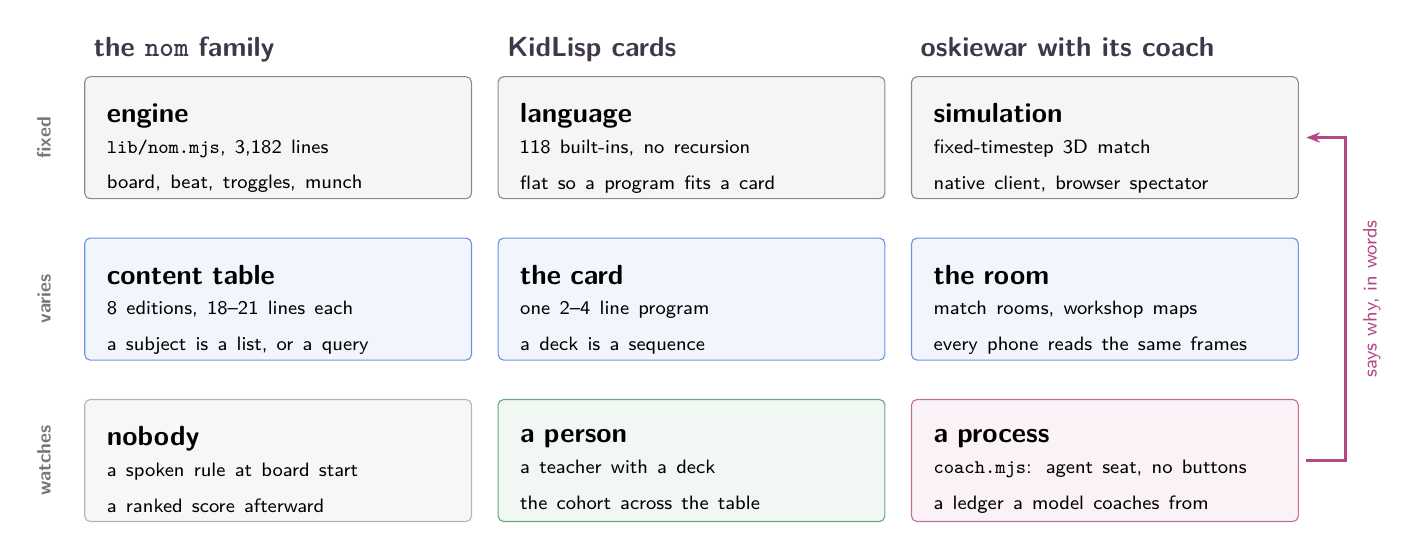
\begin{tikzpicture}[
  every node/.style={font=\sffamily},
  cell/.style={draw=acgray!55, rounded corners=2pt, fill=white, align=left, anchor=north west,
    minimum height=1.55cm, text width=4.35cm, inner xsep=8pt, inner ysep=6pt, text depth=0.62cm},
  engine/.style={cell, draw=acdark!60, fill=acdark!5},
  table/.style={cell, draw=acblue!70, fill=acblue!6},
  none/.style={cell, draw=acgray!55, fill=acgray!6},
  human/.style={cell, draw=acgreen!75, fill=acgreen!7},
  machine/.style={cell, draw=acpink!80, fill=acpink!7},
  head/.style={font=\sffamily\bfseries, anchor=base west, text=acdark},
  side/.style={font=\scriptsize\sffamily\bfseries, anchor=east, text=acgray},
  lab/.style={font=\scriptsize\sffamily, text=acpink, anchor=west, inner xsep=0pt}
]
  \def\colA{0}\def\colB{5.25}\def\colC{10.5}
  \def\rowA{0}\def\rowB{-2.05}\def\rowC{-4.10}

  % column heads
  \node[head] at (\colA,0.25) {the \texttt{nom} family};
  \node[head] at (\colB,0.25) {KidLisp cards};
  \node[head] at (\colC,0.25) {oskiewar with its coach};

  % row: fixed engine
  \node[engine] at (\colA,\rowA) {\textbf{engine}\\[-1pt]{\scriptsize \texttt{lib/nom.mjs}, 3,182 lines}\\[1pt]{\scriptsize board, beat, troggles, munch}};
  \node[engine] at (\colB,\rowA) {\textbf{language}\\[-1pt]{\scriptsize 118 built-ins, no recursion}\\[1pt]{\scriptsize flat so a program fits a card}};
  \node[engine] at (\colC,\rowA) {\textbf{simulation}\\[-1pt]{\scriptsize fixed-timestep 3D match}\\[1pt]{\scriptsize native client, browser spectator}};

  % row: swappable table
  \node[table] at (\colA,\rowB) {\textbf{content table}\\[-1pt]{\scriptsize 8 editions, 18--21 lines each}\\[1pt]{\scriptsize a subject is a list, or a query}};
  \node[table] at (\colB,\rowB) {\textbf{the card}\\[-1pt]{\scriptsize one 2--4 line program}\\[1pt]{\scriptsize a deck is a sequence}};
  \node[table] at (\colC,\rowB) {\textbf{the room}\\[-1pt]{\scriptsize match rooms, workshop maps}\\[1pt]{\scriptsize every phone reads the same frames}};

  % row: watcher
  \node[none] at (\colA,\rowC) {\textbf{nobody}\\[-1pt]{\scriptsize a spoken rule at board start}\\[1pt]{\scriptsize a ranked score afterward}};
  \node[human] at (\colB,\rowC) {\textbf{a person}\\[-1pt]{\scriptsize a teacher with a deck}\\[1pt]{\scriptsize the cohort across the table}};
  \node[machine] at (\colC,\rowC) {\textbf{a process}\\[-1pt]{\scriptsize \texttt{coach.mjs}: agent seat, no buttons}\\[1pt]{\scriptsize a ledger a model coaches from}};

  % side labels
  \node[side] at (-0.3,-0.78) {\rotatebox{90}{fixed}};
  \node[side] at (-0.3,-2.83) {\rotatebox{90}{varies}};
  \node[side] at (-0.3,-4.88) {\rotatebox{90}{watches}};

  % the feedback arrow on the coach column: ledger back to the player as language
  % boxes are 4.35cm text width + 2 x 8pt inner xsep = 4.91cm wide
  \draw[-{Stealth[length=5pt]}, draw=acpink, line width=0.9pt]
    (\colC+5.02,\rowC-0.78) -- ++(0.5,0) |- (\colC+5.02,\rowA-0.78);
  \node[lab, rotate=90, anchor=north] at (\colC+5.62,\rowB-0.78) {says why, in words};
\end{tikzpicture}
}
\caption{The seam the three objects share, read row by row. Every object has a fixed engine and a swappable table of content. The bottom row is the one the two traditions leave under-built and the one on which the objects differ most: the drill has no watcher, the card has a person, the coach has a process that keeps a ledger for a model. The arrow on the coach column is the only feedback path that goes back to the learner as language rather than as a score.}
\label{fig:seam}
\end{figure*}

Figure~\ref{fig:seam} draws what the three sections have in common. The \code{nom} paper found a seam between a mechanic that stays and a subject that varies, and called it an engineering result. The cards paper found the same seam in a language: the built-ins stay, the program varies, and the card is the unit of variation. oskiewar has it too, with match rooms and workshop-edited maps as the table and a fixed-timestep simulation as the engine. That much is ordinary software architecture.

What the comparison adds is the third row. In each object, what happens \emph{after} a correct move is where the teaching lives, and each handles it differently. The drill's feedback is inside the engine: clear the square, play the note, speak the translation. It is immediate, integrated in Habgood's sense, and mute about \emph{why}. The card's feedback is a person, which is the best kind and the least scalable. The coach's feedback is a process that has been given the whole match and asked to explain it later, in words, to the player, through a model. It is the first of the three that can say why.

I think this is the actual answer to the old question. Games teach when the answer is the thing you do (the drill got that right in 1986) and when someone outside the game is keeping a record of more than the score (the drill never got that, and the kit could only get it by hiring a teacher). The seam that makes a drill cheap to extend is the same seam that lets a watcher be attached without touching the game. \code{coach.mjs} attached to oskiewar in one file. The \code{nom} engine emits the same events (a munch, a miss, a death, a rule) and has no seat for anyone to sit in. That is the next table to write.

\section{What a School Would Need}
\label{sec:school}

\emph{Get Closed Source Out of Schools} argued that the 50 million Chromebooks in American classrooms are gateways denied, and pointed at Kerala, where the KITE program moved 16,000 public schools to free software in 2007 and now runs it on more than 300,000 machines~\citep{scudder2026openschools,kite2024gnulinux}. The three objects here are, in that argument's terms, well shaped for a school and not yet ready for one.

Well shaped, because a \code{nom} game is a URL. \code{aesthetic.computer/numbnom} runs in a Chromebook's browser with no install, no account, and no download, and \code{source numbnom} returns its code, which is Papert's demand and Illich's (that the tool be convivial, inspectable, and the learner's own) met in one command~\citep{illich1971deschooling,scudder2026pieces}. A teacher who wants \emph{eat the noble gases} needs a list, not a programmer.

Not ready, for three reasons the record already contains. First, the license: the repository declares ISC in its manifests and ships no license file, which on Stallman's map leaves it source-available rather than free, and a district's procurement office will notice~\citep{scudder2026freevsopen}. Second, the ladder: ranked scores require a signed-in handle, and this paper did not audit what an \ac{} account asks of a child or whether any age gate exists. A school deployment would have to run without the ladder or answer that question first. Third, the watcher: the only object with a machine watcher is the one with no educational intent, and it feeds a model whose inference someone pays for. Denny and colleagues' survey of computing education after generative AI is clear that the tutor-in-a-model is arriving whether classrooms want it or not~\citep{denny2024computing}; the coach is a small, honest version of that arrival, and it is not yet attached to the drill a child would actually play.

\section{Ethics, Privacy, and Limitations}
\label{sec:limits}

No children were studied. No learning outcome was measured. Every claim here is about artifacts and their history, and the paper should be read as an argument about design supported by a repository, not as evidence that anyone learned anything. The one classroom in the record was a graduate seminar whose cohort were critics, not pupils, and whose feedback is not quoted here.

The screenshots were taken by a headless browser with no player present; they show the opening state of each board, not play. \code{artnom} could not be captured this way, because its museum thumbnails did not load in the headless environment, and it is described from source instead.

The coach ledger records match telemetry against a player's handle and hands it to a third-party model. Anyone attaching it should know that. The \code{nom} ladder stores handles and best runs on the project's server. \code{artnom} redistributes no images; it links to the museum's own server and records each object's rights, which is the right shape, and this paper did not verify every record.

The literature sample is small and Anglophone in the main; Freire, Vygotsky, and the Kerala program are the non-Western anchors, and Ito, Ainsworth, Kafai, Peppler, Rusk, Brennan, Compton, Salen, Steinkuehler, and hooks carry the women-authored share, which the house audit asks a paper to check. Gee's principles and Malone's ingredients are cited as their authors state them; the replication literature on both is thinner than their citation counts suggest, and Habgood and Ainsworth's effect is one study with one game.

Finally, the seam is a reading, not a law. Three objects from one project by one author will share structure because one person built them. Whether a drill, a card, and a coach from three unrelated projects would show the same three rows is exactly the kind of claim this paper is not entitled to make.

\section{Conclusion}
\label{sec:conclusion}

The drill and the kit were never enemies. The drill got one thing right in 1986, that the answer should be the thing you do, and the \code{nom} family shows that a drill built on a clean seam grows by tables: four new subjects in three months, one of them a museum catalog, and the two gaps its own paper listed closed within a day and within two months. The kit got the other thing right, that the learner should be the author, and the card shows what that costs: a flat language, a low ceiling, and a person on the other side of the table.

What neither tradition built is the watcher, and the one place it got built here was a fighting game with no educational intent, in one file, in a way that never touches the controls. That is the finding. Put the fixed part in an engine, put the varying part in a table, and leave a seat outside the circle for someone to keep a record of more than the score. The \code{nom} engine has the first two. The seat is the next thing to add, and it is one file.

\bibliographystyle{plainnat}
\setlength{\bibsep}{0.6pt plus 0.2ex}
{\footnotesize\bibliography{references}}

\vspace{0.8em}
\begin{center}
\footnotesize\sffamily\color{acgray}
Revision \paperrev\;\textperiodcentered\;\texttt{\paperhash}\;\textperiodcentered\;
\href{https://papers.aesthetic.computer/gaming-education-26-arxiv.pdf}{papers.aesthetic.computer/gaming-education-26-arxiv}
\end{center}

\end{document}
